\documentclass{/workdir/classes/summary}

\graphicspath{{figures/}}

% タイトルの項目
\title{正常音の空間マッピングに基づく石油精製プラント内の異常の検知と位置推定}
\studentid{47-236699}
\author{田中 健太郎}
\supervisor{山下 淳 教授}
\abst{
  In this paper, we propose a method to detect and localize abnormal sounds in an oil refinery plant by mapping normal sounds and leveraging the difference between observed and predicted normal acoustics. By constructing a neural network that learns the spatial distribution of normal sounds, we can compare incoming audio signals with predicted ones and identify anomalies. Our approach also calculates the distance between the robot and potential sound sources using sound pressure attenuation, enabling more accurate localization through triangulation. Experiments conducted in both indoor and actual refinery environments show promising results, detecting abnormal sounds and accurately estimating their positions even under high background noise.
}
\kwd{Abnormal Sound Detection, Oil Refinery Plant, Neural Network, Sound Localization}

\begin{document}
\maketitle

\thispagestyle{mypagestyle}
\pagestyle{mypagestyle}

\section{序論}

近年,地球温暖化の進行を抑えるため,カーボンニュートラルの実現が求められている.しかし石油をはじめとする化石燃料は,
将来的にもエネルギー源として重要な役割を果たすと考えられる.

石油の精製は,ガソリン,ディーゼル燃料,ジェット燃料などの輸送用エネルギー資源だけでなく,プラスチック,化学肥料,医薬品,合成繊維など,幅広い化学製品を生み出すために欠かせない工程である.その中心的役割を担うのが石油精製プラントであり,施設内にはポンプ,熱交換器,蒸留装置,配管など多種多様な装置が複雑に組み合わさって存在している\cite{Shvindin2008A}.
これらの装置が適切に稼働することで,高品質なプロダクトが安定して供給され,産業や社会の基盤を支えている.

また,保守作業はどの産業においても重要な要素であり,石油精製プラントも例外ではない.
設備は老朽化や環境条件による劣化で故障することがあり,その結果,操業停止による生産遅延,修理費の増加などの損失が発生する.
さらに,石油精製プラントでは可燃性物質を多数扱うため,他の産業施設に比べて火災や爆発など重大な事故が発生するリスクが高く,その被害は甚大になり得る\cite{Tang2021105623}.
こうしたリスクを低減するためには,設備の異常を早期に発見し,適切な対策を講じることが求められる.

現状では,石油精製プラント内の設備点検は専属の現場作業員が定期的な巡回で行い,視覚・聴覚・嗅覚・触覚による異常の有無の確認が基本である.
こうした点検は1日に4~5回実施され,昼夜を問わず行われているため,夜間作業による負担や,高齢化による熟練人材の不足,熟練度の差による点検品質のばらつきといった様々な課題が生じている.
これらの理由から,プラント内点検の自動化が求められている.

プラント内点検の自動化には主に2つのアプローチがあり,1つは固定センサを用いた点検,もう1つは移動ロボットを用いた点検である.固定センサを用いた例として,Lv らが提案しているマイクによるギアやポンプなどの異常音検知手法が挙げられる\cite{Lv2023Overview}.固定センサ方式は常時監視が可能である一方,多数の可燃性物質を扱うプラント内では通信線を含むすべての機器を防爆仕様とする必要があり,導入コストが高くなる.また,広大なプラント全体を監視するためには多数のセンサを設置しなければならないため,設置・維持コストもかさむ.
そのため,移動ロボットを用いた点検が注目されている.
このような理由から,本研究では移動ロボットを用いた点検に着目する.

現在,プラント内には多種多様な機器が存在し,それぞれの機器から発生しうる異常に応じた感覚器官を用いて異常の検出が行われている.
その中でも聴覚を用いた点検は非常に重要である.
というのも視覚を用いた点検では遮蔽によって筐体内部の情報を取得することができないが,聴覚は筐体内部の情報を取得することができるためである.
また,触覚と違い,対象機器へのコンタクトレスな点検が可能である.
そのため聴覚を用いた点検には大きな意義があり,本研究では聴覚を用いた異常音検知に着目する.

プラント内の音響点検を行うにあたって,プラント内特有の課題が存在する.
まず,プラント内では機器が密集しており,異常音の検出のみならず位置推定までが求められる.
更に,プラント内の音響点検の対象となるベアリングは傷の深さや位置に応じて種多様な異常音が存在し,そのデータを取得することは困難である.
それを踏まえ,本研究では正常音のデータのみを学習に用いて移動ロボットを用いてプラント内を走行しながら異常音を検知し,その異常音が発生している機器の位置を推定する手法の構築を目指す.

近年の異常検知手法には,教師あり異常検知と教師なし異常検知が存在する.教師あり異常検知(Supervised AD)では,異常か正常かのラベルが付与されたデータを用いることで,異常の特徴を直接把握でき,高い精度を発揮しやすい.ただし,異常事例が極端に少ない場合にはクラス不均衡問題が生じ,性能が低下する課題がある.一方,教師なし異常検知(Unsupervised AD)は正常データのみを用いてモデルを学習するため,異常データを事前に十分に集めにくい状況に適している.
異常データを十分に集めにくい状況は本研究で対象とするプラント内の音響点検に関しても同様であり,教師なし異常検知のアプローチが有効であると考えられる.

さらに,移動ロボットにマイクを搭載して異常音を検知する研究も行われている.先に述べたように,移動ロボットを用いた手法は空間的な情報を使用できるため,異常の位置推定のタスクに用いられることが多い.
ただし,Song ら\cite{9023943}が提案する手法では,異常音を抽出するためのフィルタを手作業で設計しており,多様な異常音に対応するには限界がある.また,Fujita ら\cite{10202270} は空間をグリッドに分割して各グリッドで正常音を学習するが,グリッドの解像度でしか異常音の位置を推定することができない.
本研究では,上述の課題を踏まえ,移動ロボットを想定した異常音の教師データを用いずに多様な異常を検知し,さらに異常位置を推定できる手法の構築を目指す.
\section{提案手法}

\subsection{提案手法のコンセプト}
従来手法では異常音の抽出にヒューリスティックに設計したフィルタリングを用いるため,多様な異常音に対応することができなかったり,空間的に離散的なモデルを用いているため,異常の位置推定が困難であった.
本研究ではこれらの課題の解決を目的として,移動ロボットが取得する音響信号を基に,正常音を空間的にマッピングし,
マッピングされた正常音との誤差を用いて異常音を検出し,検出された異常音のエネルギーの大きさに基づいて異常音の位置を推定する手法を提案する.

\subsection{提案手法の流れ}
提案手法のフローチャートを\reffig{fig:flowchart}に示す.
まず,異常音源を含まない経路で移動ロボットを走行させることで,正常時の座標と音の関係をモデルに学習させる.
運用時には,学習したモデルを用いて検査対象となる経路を走行させ,閾値処理により経路内の異常音源の有無を判別したのち,異常音源が確認された場合には,その位置を推定する.
\begin{figure}[t]
  \centering
  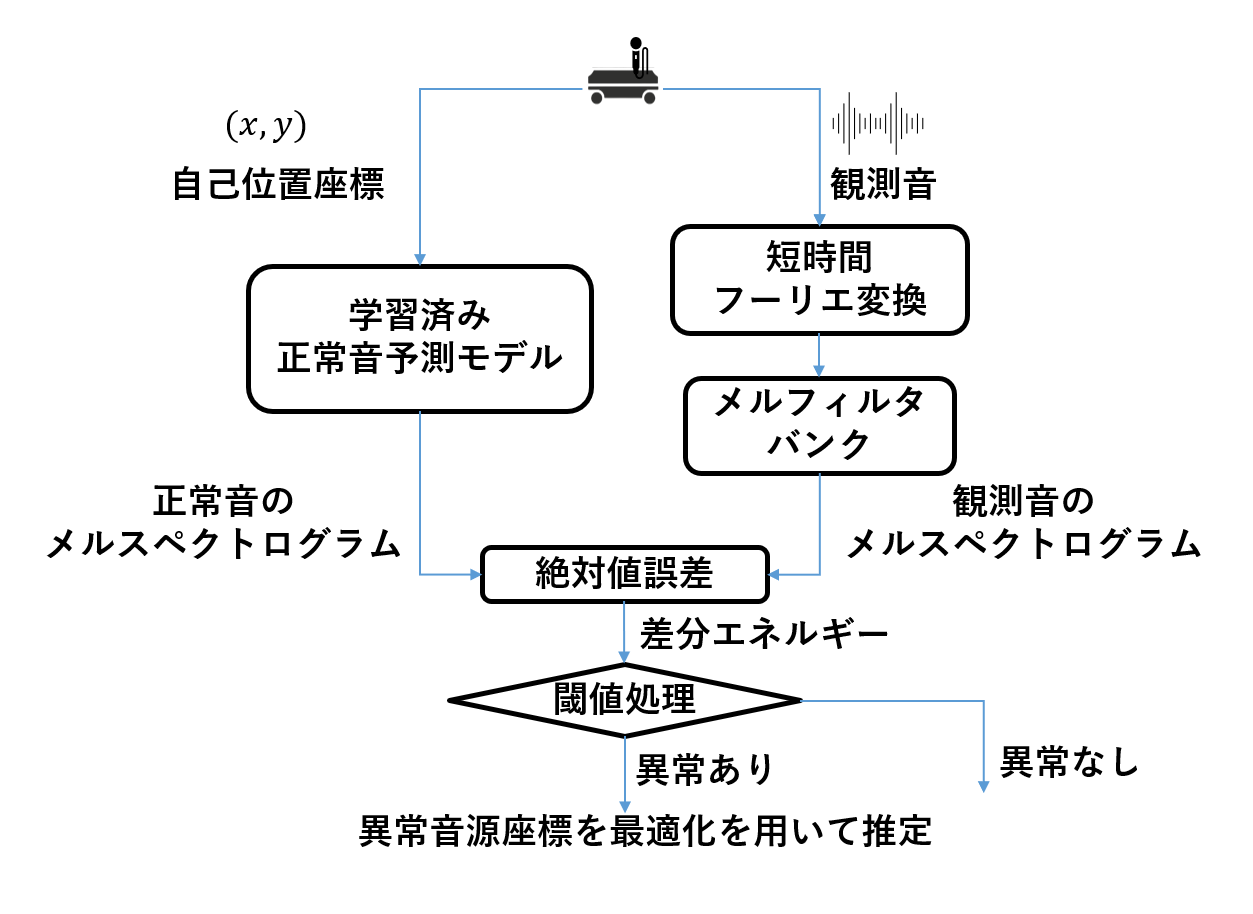
\includegraphics[keepaspectratio, width=1.0\linewidth]{flowchart.png}
  \caption{提案手法のフローチャート}
  \label{fig:flowchart}
\end{figure}


\subsection{正常音のマッピング}
ボットの位置座標とマイク出力の関係を学習するために,ニューラルネットワークを用いる.
ニューラルネットワークは近年,入力データと出力データのあいだにある複雑な関係をとらえる能力に優れていることが知られている.
本研究ではロボットの位置座標を入力とし,対応するメルスペクトログラムを出力するネットワークを構築する.
出力としてメルスペクトログラムを用いる理由は,その算出過程で短時間フーリエ変換を行い,周波数領域の情報から回転機器の定常的な特徴をとらえやすいためである.しかし,ウィンドウ関数を用いて短時間のサンプルに分割する都合上,サンプル間の相関が失われてしまう.一方,実環境では隣接する位置のあいだで音データに連続性がある.
この関係性をモデルに反映させるため,本研究ではSharpness-Aware Minimization(SAM)\cite{sam}を用いて学習を行う.
SAMは重みの変化に対する損失関数の変動を抑制することで汎化性能を高める最適化手法であり,ロボットの位置に応じてモデルの出力がより滑らかに変化することが期待される.
\subsection{異常の位置推定}
以下では、ロボットが取得した音声データを用いて異常音源の位置を推定する手法について述べる.
予測した正常音との誤差から各地点での異常音エネルギーを算出することができる.
ここで,音源からの音圧レベルの減衰が距離の2乗に反比例する性質を利用し,観測地点ごとの異常音エネルギー値から音源までの距離を算出する.これにより複数地点のデータを基に三辺測量を用いて音源の位置を推定する.

しかし、実環境ではノイズなどにより距離推定に誤差が生じるため、最適化アルゴリズムを活用して誤差を最小化する手法を採用する.具体的には,エネルギー値に基づいた重みづけを損失関数に取り入れ、音源に近い地点のデータを重視した最適化を行う.これにより,ノイズの影響を軽減しながら異常音源の位置を高精度に推定することを目指す.


\section{検証実験}
\subsection{屋内実験}
本実験では,プラント内環境を模擬した環境を実験室内で作成し,提案手法の有効性を検証した.
複数のギアボックスを設置し,騒音環境を再現した状態で実験を行った.
マイクロホン(Shure SM11)とZoom P4を用い,48kHzで音響を収録した.
移動ロボットにARマーカーを搭載し,Logicool C925eカメラによってロボットの位置を取得しながら音響データを取得した.
タミヤ製教育工作キットのギアボックスを複数用意し,回転機器を模擬した.
正常状態のギアボックスを用いてロボットを走行させ,正常音を収集したのち,1つのを対象にギアボックスを傾けることで異常音を発生させ,異常状態の音声を収集した.
異常状態の経路は異常のギアボックスの位置を変えて2回実施し,異常音源の位置を推定した.
録音データの低周波帯域にはロボット振動によるノイズが含まれていたため,1000Hz未満の周波数帯を除去した.
メルスペクトログラム変換には,ウィンドウ幅として65536サンプルを用いた.
\subsection{屋外実験}
本研究では,実験室内での評価に加え,より実環境に近い条件下で提案手法の性能を検証するため,石油精製プラント内での屋外実験を実施した.
実験は,\reffig{fig:field_environment}に示す石油精製プラントの稼働エリアの一角で実施した.
このエリアには,連続的に作動するポンプ類や定期的に圧力を放出するバルブ類など,複数の騒音源が点在している.
自己位置の推定はロボットの車輪に搭載したエンコーダを用いて行い,音響データの取得は屋内実験と同様に行った.
定期的に圧力を放出するバルブ類が点在している.作業日当日もプラント全体が通常稼働中であり,背景騒音は実験室よりも格段に大きい環境であった.
240 BPMで金属棒を打ち鳴らす周期的な音源と,インパクトドライバによる連続衝撃音を異常音源として用いた. これら2種類の異常音源を\reffig{fig:field_environment}の地点Aと地点Bに配置し,通過ルートを複数回走行してデータを取得した.それぞれの走行における異常音源の配置を表\reftab{tab:abnormal_sound_jp}に示す.
 なお,当日は種々の制約により,異常音源の正確な座標記録は行えなかった.

\begin{figure}[t]
  \centering
  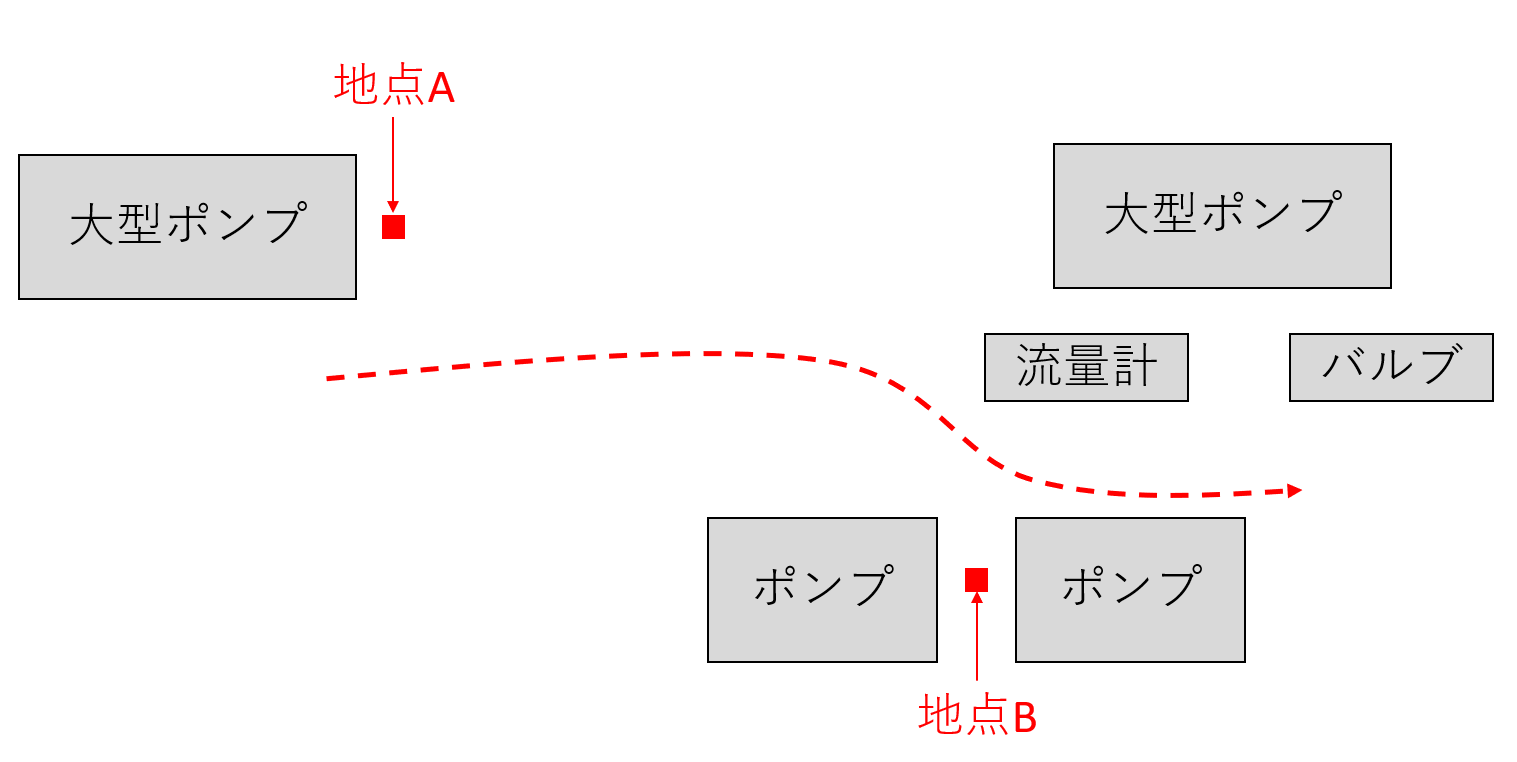
\includegraphics[keepaspectratio, width=1.0\linewidth]{field_environment.png}
  \caption{屋外実験における実験環境}
  \label{fig:field_environment}
\end{figure}

\begin{table}[htbp]
  \centering
  \caption{各パスにおける各地点の異常音源}
  \label{tab:abnormal_sound_jp}
  \begin{tabular}{c|c|c}
  \hline
   & \textbf{地点A} & \textbf{地点B} \\ \hline
  \textbf{1回目} & 金属棒を打撃 & インパクトドライバ \\
  \textbf{2回目} & インパクトドライバ & 金属棒を打撃 \\ \hline
  \end{tabular}
\end{table}

\section{実験結果・考察}
\subsection{屋内実験}
\reffig{fig:observed_mel}と\reffig{fig:predicted_mel}に,正常状態における観測されたメルスペクトログラムと予測されたメルスペクトログラムをそれぞれ示す.
\begin{figure}[t]
  \centering
  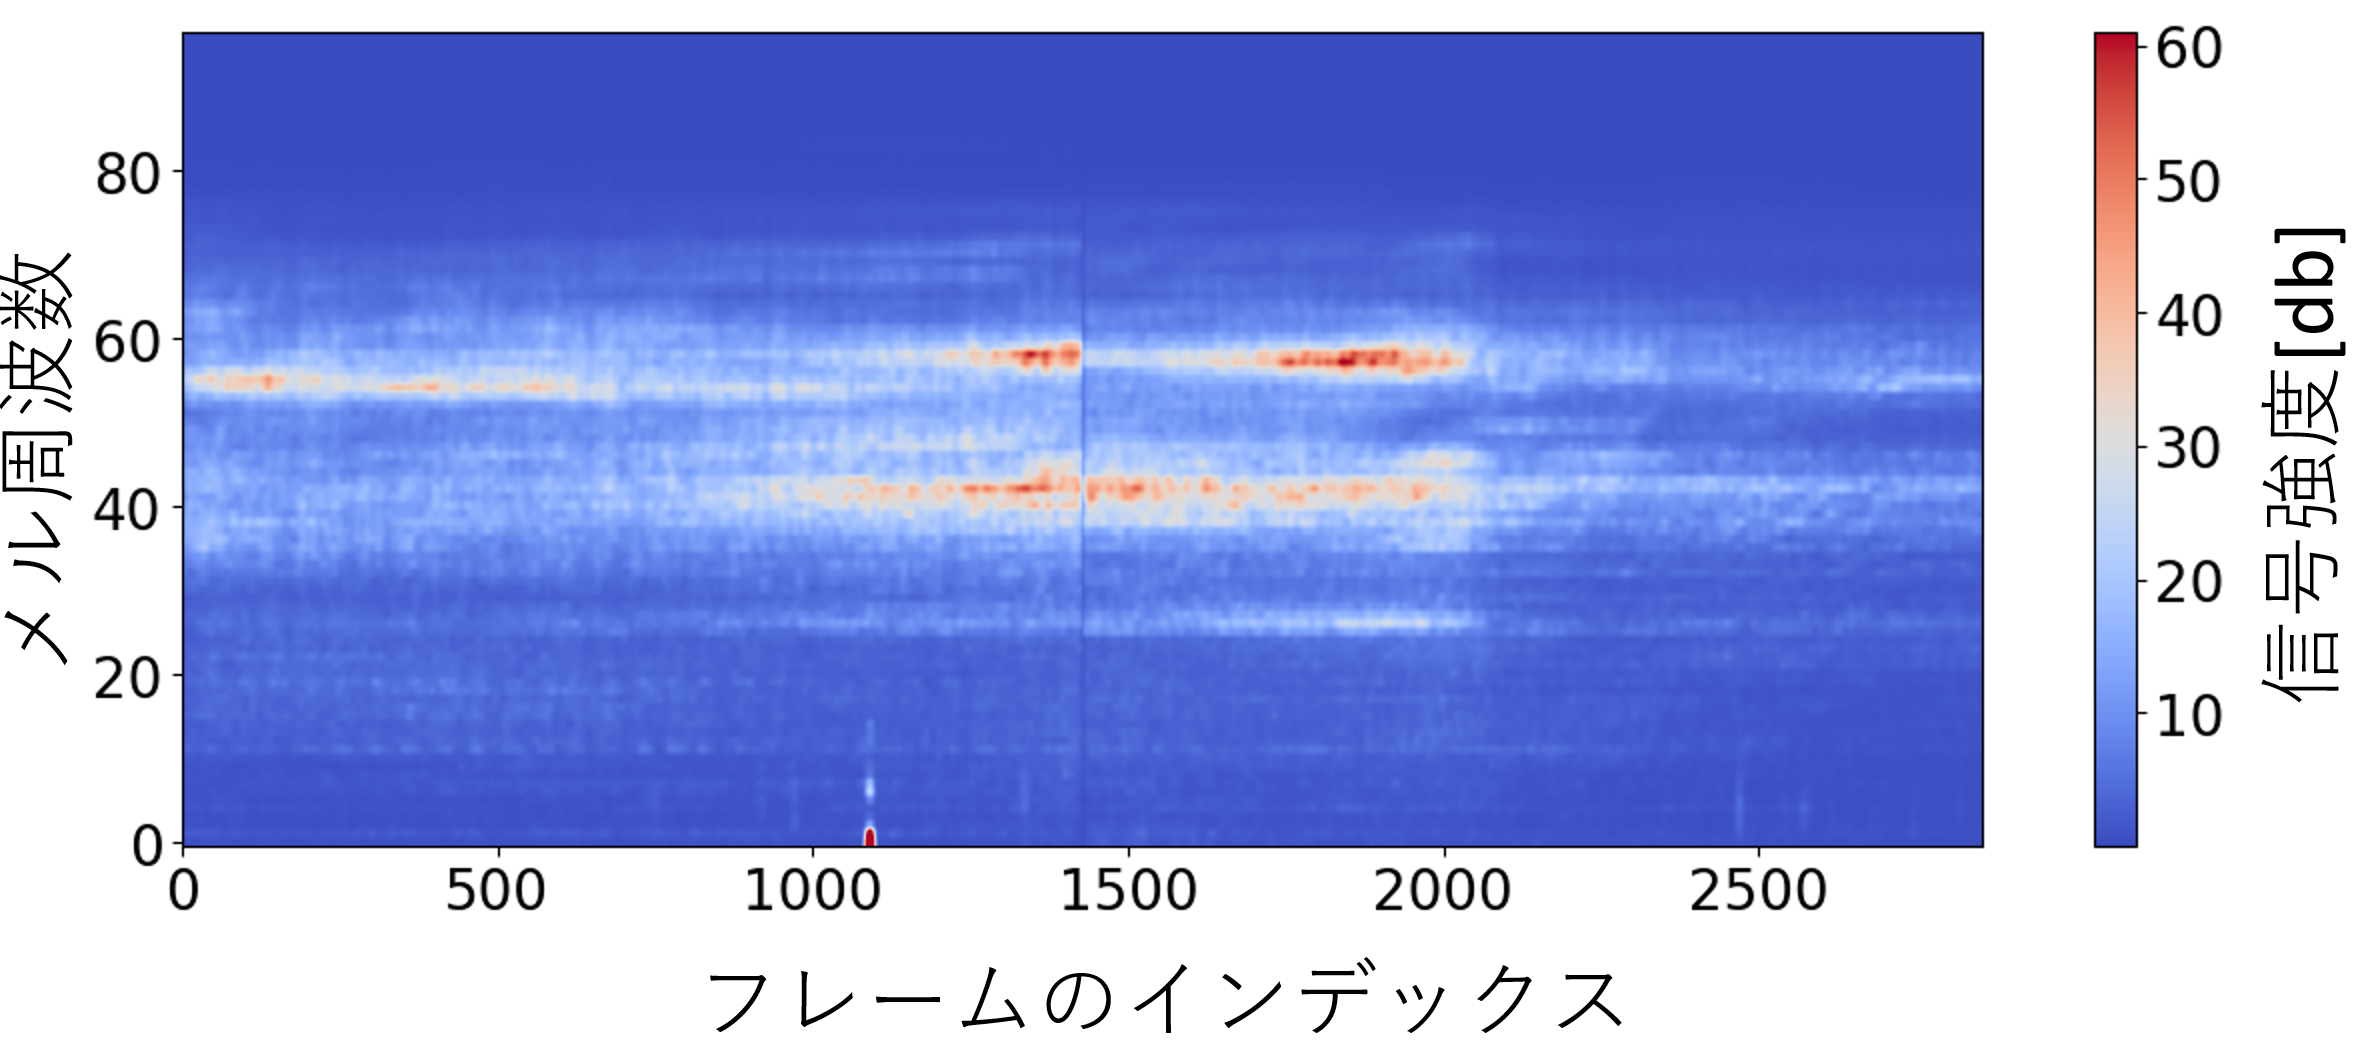
\includegraphics[keepaspectratio, width=1.0\linewidth]{observed_mel.png}
  \caption{観測されたメルスペクトログラム}
  \label{fig:observed_mel}
\end{figure}

\begin{figure}[t]
  \centering
  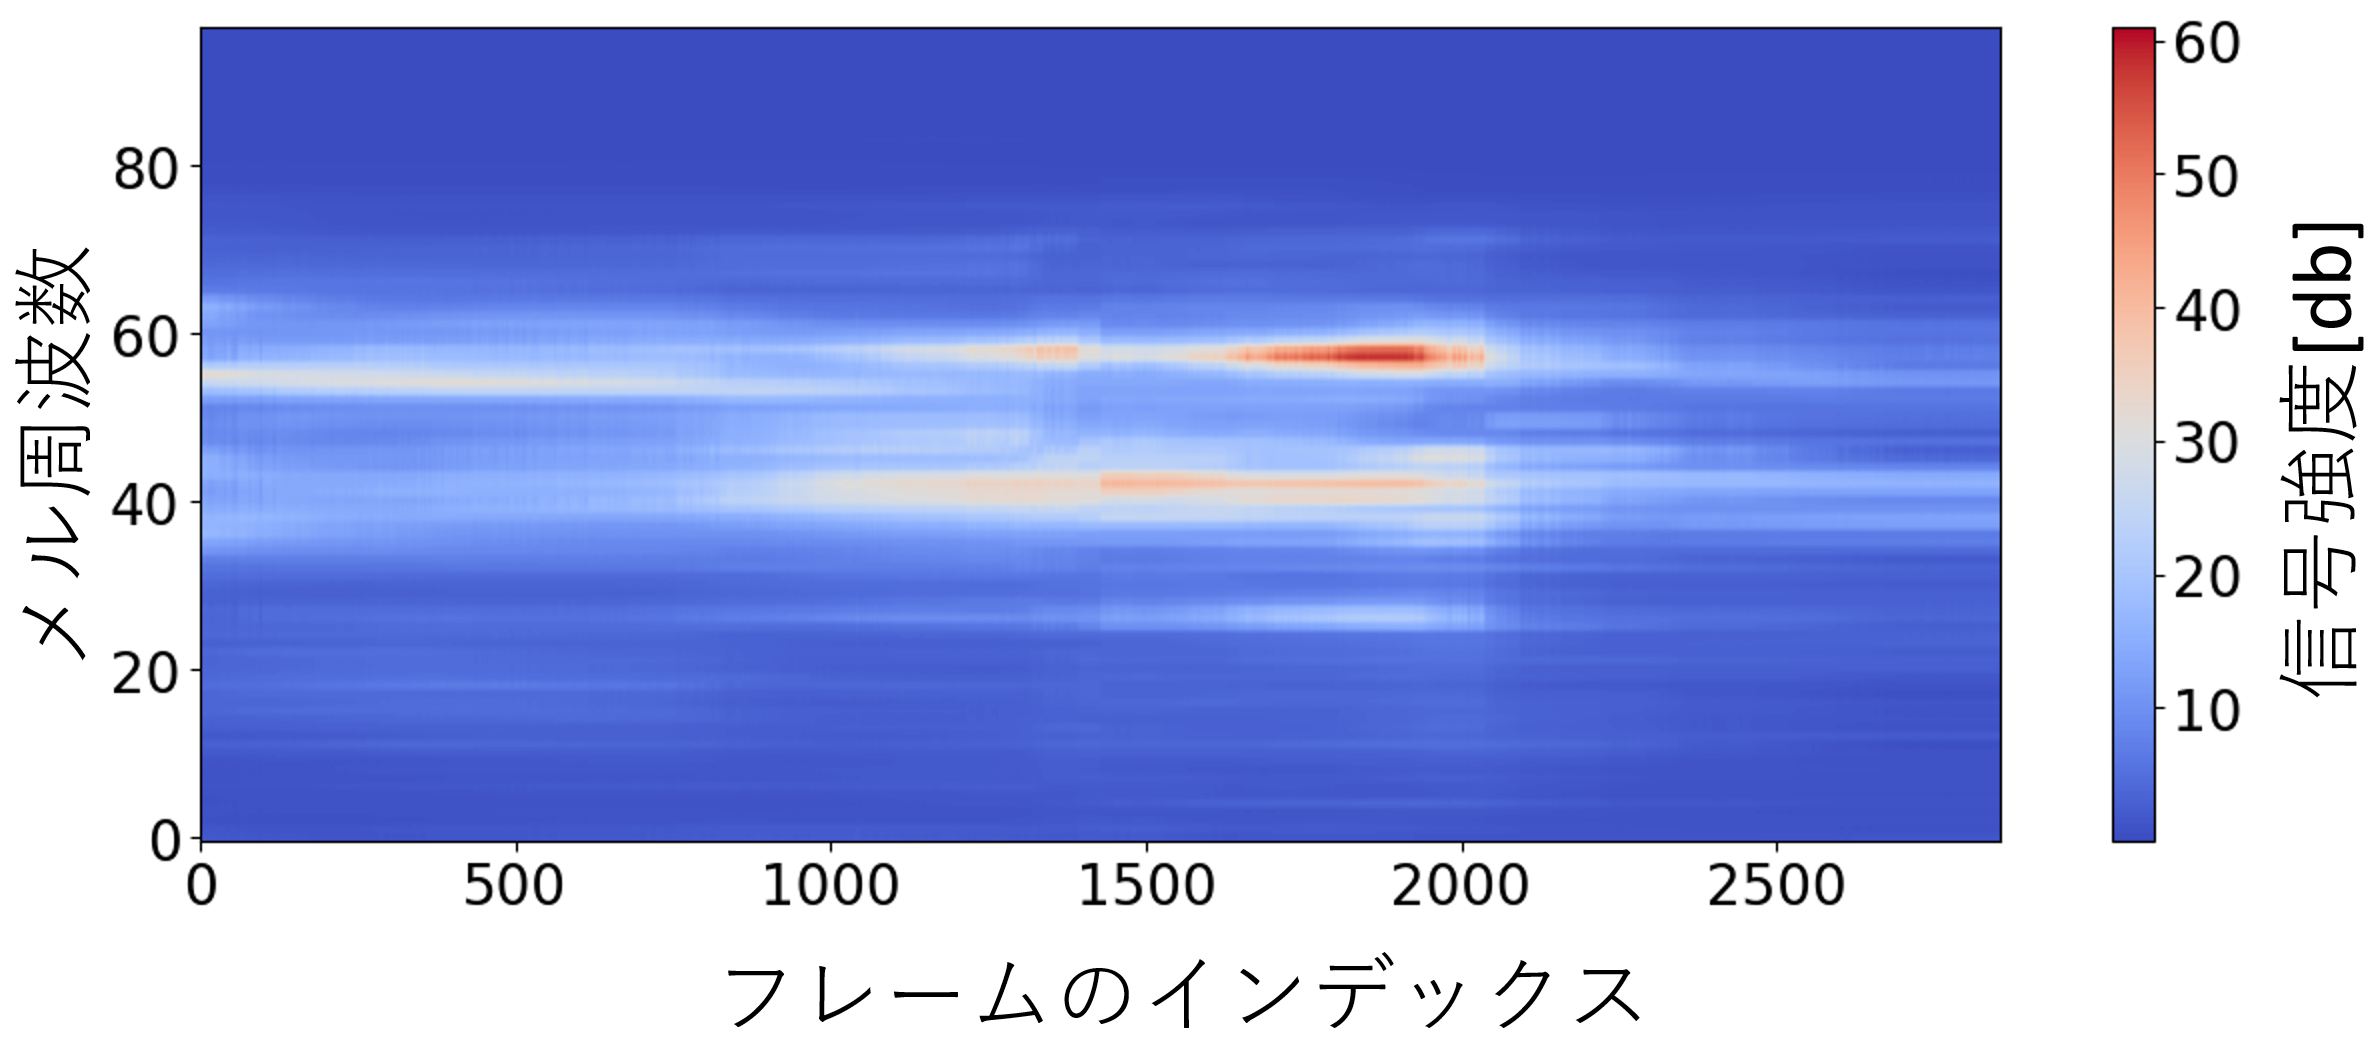
\includegraphics[keepaspectratio, width=1.0\linewidth]{predicted_mel.png}
  \caption{予測されたメルスペクトログラム}
  \label{fig:predicted_mel}
\end{figure}
全てのフレームにおいて,正常音の特徴が正しく予測されていることがわかる.
また,ギアボックスを傾けて異常音を発生させた状態でロボットを走行したところ,正常時に比べ,異常音源周辺で予測音との差分エネルギーが大きくなることが確認された(\reffig{fig:lab_normal},\reffig{fig:lab_abnormal2},\reffig{fig:lab_abnormal7}).
経路上で異常音源に近い地点ほど差分エネルギー値が高くなり,騒音下でも異常音を検出できることが示された.
\begin{figure}[t]
  \centering
  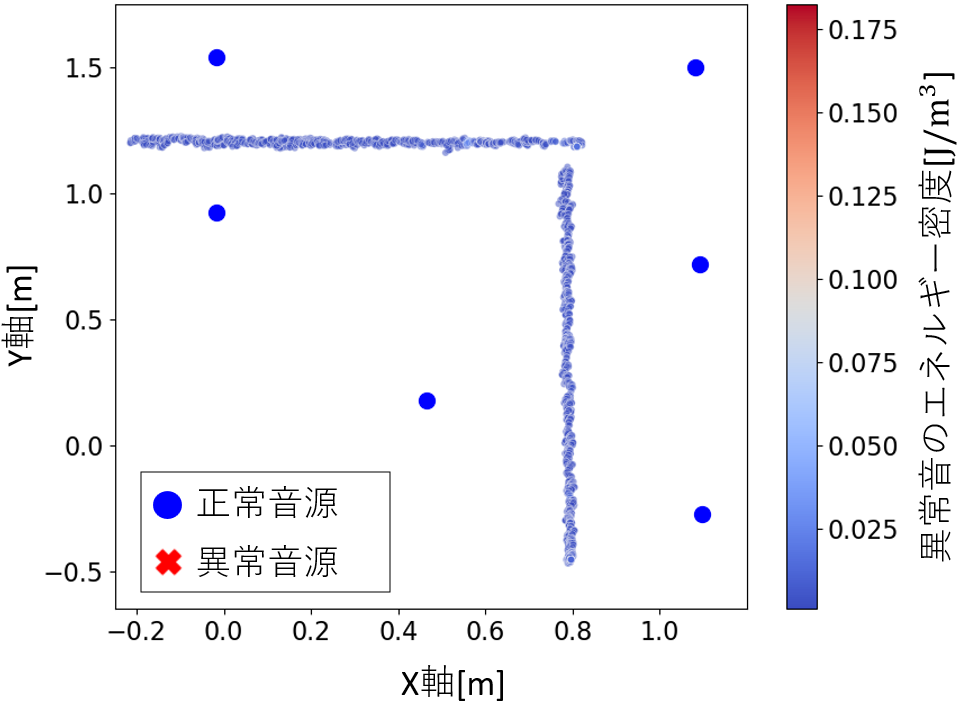
\includegraphics[keepaspectratio, width=1.0\linewidth]{lab_normal.png}
  \caption{正常状態の経路における予測音との差分エネルギーの分布}
  \label{fig:lab_normal}
\end{figure}

\begin{figure}[t]
  \centering
  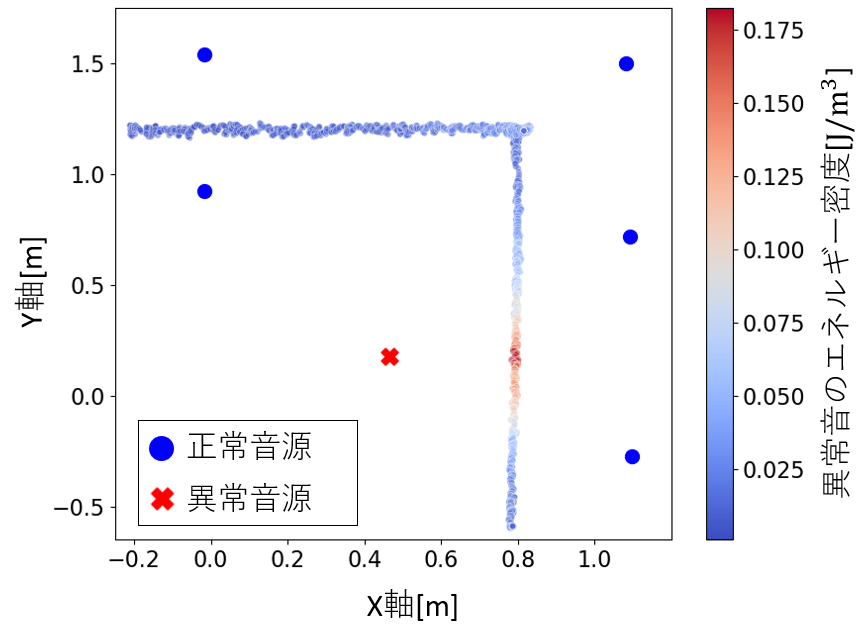
\includegraphics[keepaspectratio, width=1.0\linewidth]{lab_abnormal2.png}
  \caption{異常状態の経路における予測音との差分エネルギーの分布}
  \label{fig:lab_abnormal2}
\end{figure}

\begin{figure}[t]
  \centering
  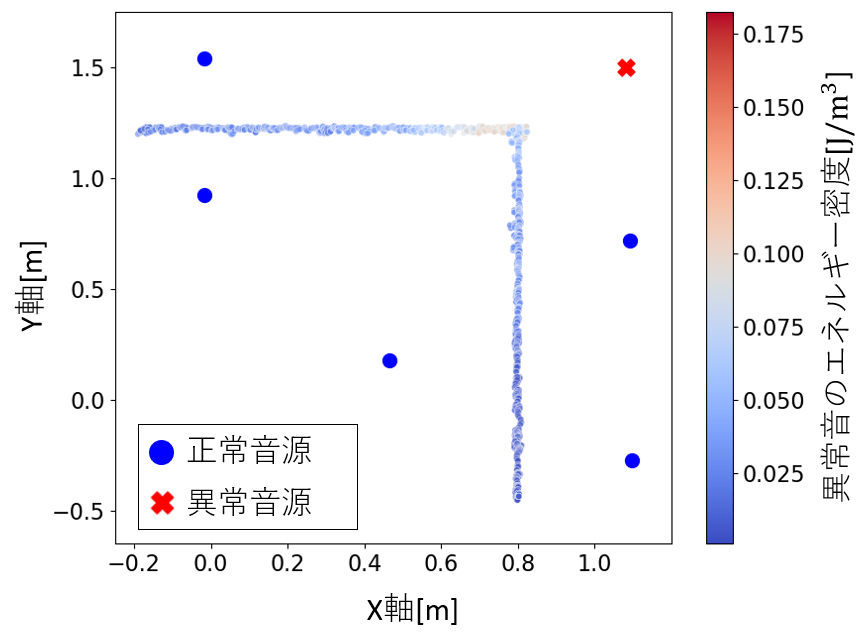
\includegraphics[keepaspectratio, width=1.0\linewidth]{lab_abnormal7.png}
  \caption{異常状態の経路における予測音との差分エネルギーの分布}
  \label{fig:lab_abnormal7}
\end{figure}


異常が検出されたエリアを対象に異常音源の位置を推定した結果を表\reftab{tab:sound_localization}に示す.
\begin{table}[h]
  \centering
  \caption{提案手法による異常音源位置推定の結果}
  \label{tab:sound_localization}
  \setlength{\tabcolsep}{3pt} % 列間のスペースを調整
  \renewcommand{\arraystretch}{0.9} % 行間を調整してコンパクト化
  \small % フォントサイズを少し小さく
  \begin{tabular}{>{\centering\arraybackslash}m{1.5cm} >{\centering\arraybackslash}m{1.5cm} >{\centering\arraybackslash}m{1.5cm}}
      \toprule
      & 位置1 & 位置2 \\
      \midrule
      真値 & (0.46, 0.18) & (1.08, 1.50) \\
      提案手法 & (0.55, 0.21) & (1.17, 1.45) \\
      誤差(m) & 0.09 & 0.10 \\
      \bottomrule
  \end{tabular}
\end{table}

真値との誤差は小さく,位置1と位置2のいずれにおいても高精度で位置推定を行うことができた.
経路上での異常音のエネルギー値には差が見られたが,最適化の重み付けにより相対的に大きいエネルギー点が正しく利用され,位置推定精度が保たれたと考えられる.
\subsection{屋外実験}
\reffig{fig:field_normal}では,殆どのサンプルが正常として判定されていることが確認された.
一方で,\reffig{fig:field_abnormal1}と\reffig{fig:field_abnormal}では,異常音源が存在するエリアにおいて異常が確認されるサンプルが増加していることが確認された.
このことから,背景騒音が高い環境下でも提案手法による異常の検出が可能であることが示された.
\begin{figure}[t]
  \centering
  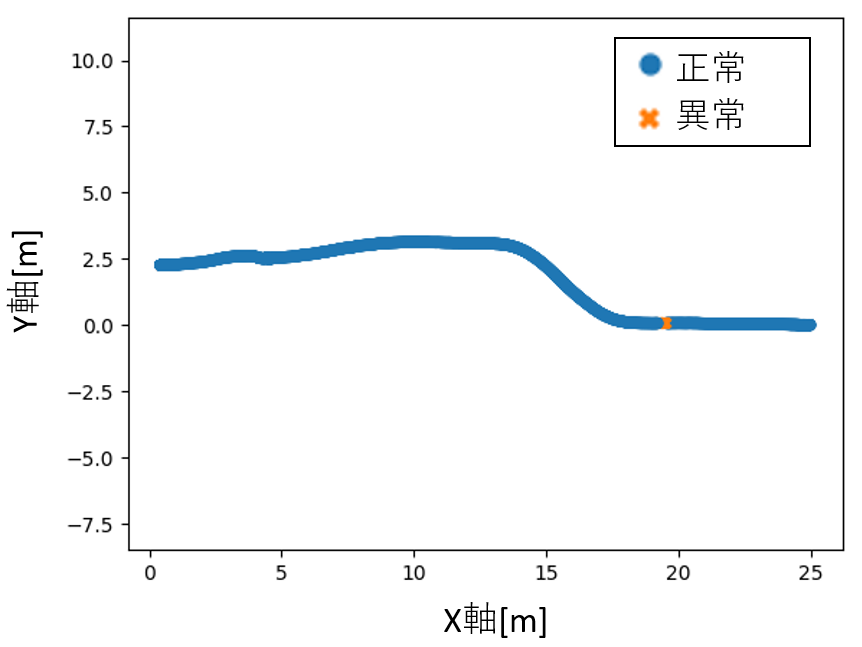
\includegraphics[keepaspectratio, width=1.0\linewidth]{field_normal.png}
  \caption{正常状態における異常検知結果}
  \label{fig:field_normal}
\end{figure}

\begin{figure}[t]
  \centering
  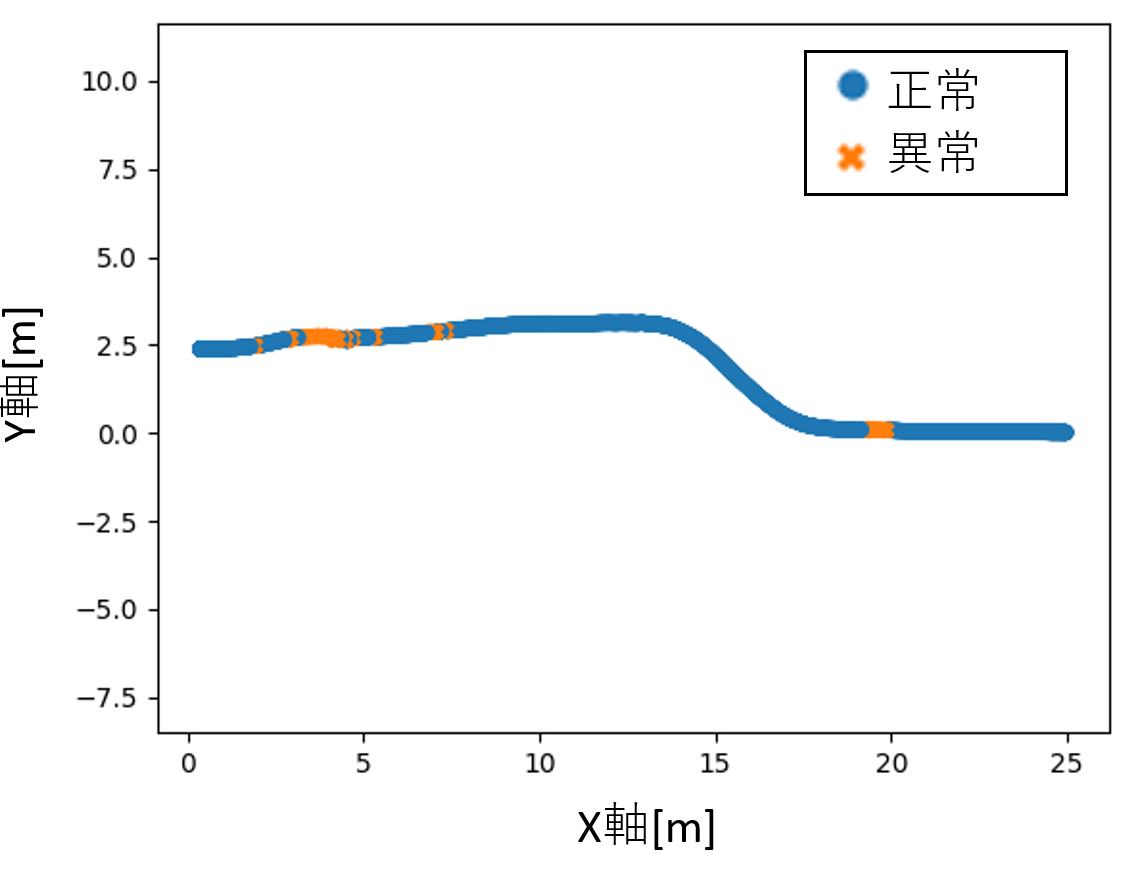
\includegraphics[keepaspectratio, width=1.0\linewidth]{field_abnormal.png}
  \caption{異常状態における異常検知結果}
  \label{fig:field_abnormal1}
\end{figure}

\begin{figure}[t]
  \centering
  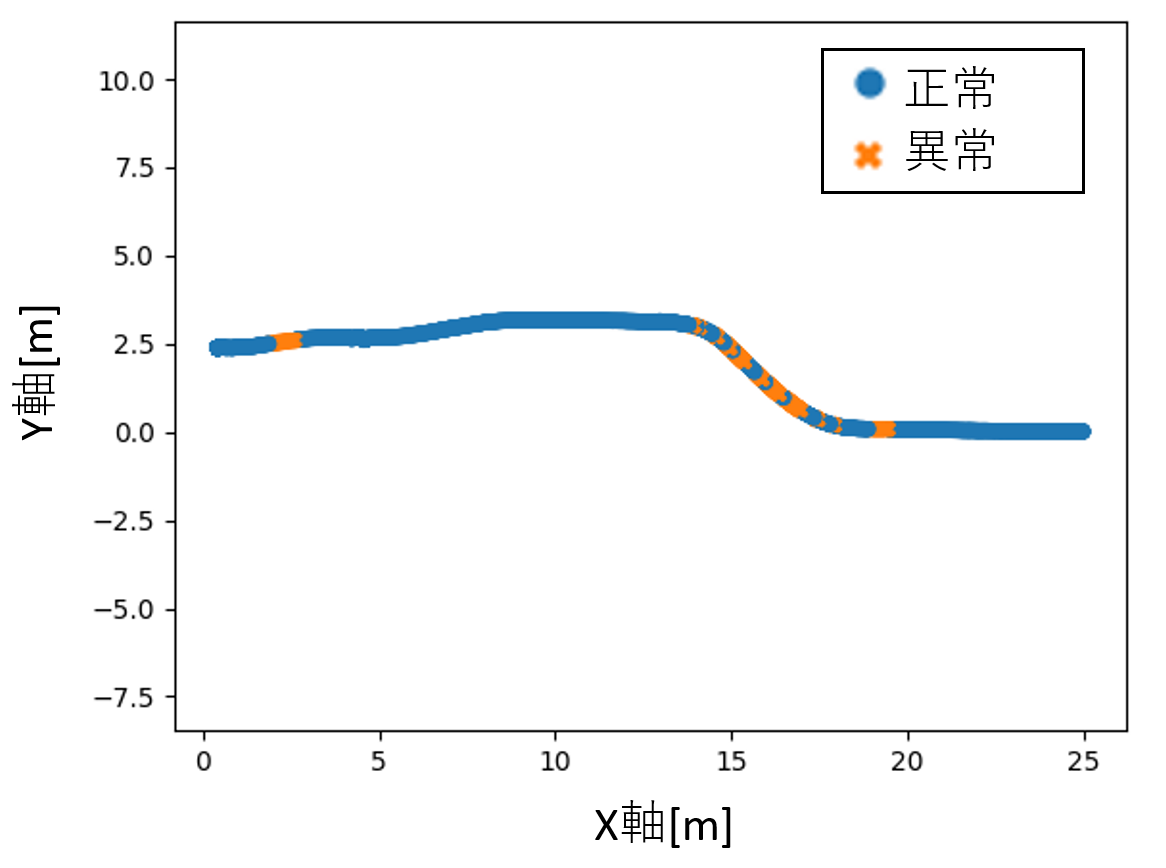
\includegraphics[keepaspectratio, width=1.0\linewidth]{field_abnormal1.png}
  \caption{異常状態における異常検知結果}
  \label{fig:field_abnormal}
\end{figure}


\section{結論}
本研究では,正常音のマッピングに基づく異常音源の検出および位置推定手法を提案した. 環境内の音響と空間的な関係を学習するモデルを作成し,実際の音と推定された音との比較をもとに検出を行う. その後,複数のパラメータを最適化することで異常音源の位置を推定する. 実験室環境での評価では,本手法が高い性能を示した. また,実際に稼働中の石油精製プラントのような非常に騒音の大きい環境でも,異常音を検出できることを確認した.

提案手法は単一の異常音源が存在することを前提としており, 通常の石油精製プラントでは複数の異常が同時に発生する可能性は低いが,万が一異常が連鎖的に発生するシナリオも想定されるため,複数の異常音源を同時に推定できる機能の実装が望まれる.
\bibliographystyle{summary}
\bibliography{sections/reference,sections/reference_web}
\end{document}
